\section{Dokumentengeschichte}
\begin{table}[h]
 \begin{tabular}{|l|l|p{4cm}|}
 \hline
 Zeitraum & PL/Autor(en) & Änderungen \\
 \hline
 Winter Semester 2017/2018 & Sefa Kanbur & Fuseki-Server
\\
\hline
 Winter Semester 2017/2018 & Gires Ntchouayang Nzeunga & 
Klassifikationshierarchie mit RDF \newline
Beziehungen mit RDF \newline
Recherchierbarkeit mit SPARQL\newline
 \\
\hline
Wintersemester 1980/81 & IHR NAME &
\\
 \hline
 \end{tabular}
 \caption{Dokumentengeschichte}
 \end{table}

\section{Aufgabe der Komponente}

Der Fuseki-Server verwaltet RDF-Dateien. Diese können in .rdf Format oder in .owl Formal in datasets hochgeladen werden.
In den datasets kann man auf die Triples in den Tabellen mit querys zugreifen. Ausgabe der Tabellen in JSON, XML, CSV und TSV als Raw Response. Raw Response auch zum direkt runterladen verfügbar. Die datasets auf den die Triples gelagert sind, kann man auch selbst erstellen unter manage datasets - > add new dataset. Nach Bedarf In-memory oder Persistens.

OHDM speichert Geoobjekte und deren Bedeutungen. Dies bedeutet, dass wir mithilfe einer Klassifikationshierarchie eine Menge von Linien interpretieren können. OHDM verfügt über eine Klassifikation, die wiederum in eine Klasse und eine Subklasse gliedert. Diese Unterteilung führt dazu, dass man eine Suche anpassend verfeinern könnte sodass die Ergebnisse in Unterkategorien gefiltert werden. Die SPARQL Schnittstelle soll die Klassifikationshierarchie in OHDM mit RDF darstellen und anschließend die Beziehungen zwischen Geoobjekten und derer Klassifikationen semantisch repräsentieren. Es soll also möglich sein, mit SPARQL nach Objekte einer Klassifikation zu suchen sowie nach allgemeineren Klassifikationen zu suchen und die Unterkategorien ebenfalls zu finden.


\section{Architektur}

\subsection{Überlick}

Wir benutzen die RDF und RDF-Schema Definition um unserer Klassifikation einer semantischen Bedeutung zu geben. RDF dient der Beschreibung von Ressourcen und die Beziehung zwischen ihnen, wobei eine Ressource „alles“ sein kann.\newline
Wir können auch in unserem Fall alles als Ressource bezeichnen. Die Klassifikation in OHDM ist eine Ressource, genauso wie die Klasse und Subklasse die sie enthaltet und die Geoobjekte die sie beschreibt. Es werden Aussagen bezüglich dieser Ressourcen betroffen, um die zwischen ihnen existierende Beziehung zu beschreiben. Solch eine Aussage stellt ein Statement dar und besteht aus einem Subjekt, Prädikat und Objekt. Das Subjekt ist immer die zu beschreibende Ressource und das Objekt der Wert der Eigenschaft, die durch das Statement beschrieben werden soll. Alle Aussagen über unsere Ressourcen werden in eine Datei gespeichert und bilden ein Datenmodell, das auf gerichteten Graphen basiert, das OHDM-Modell.

\begin{figure}
	\centering
		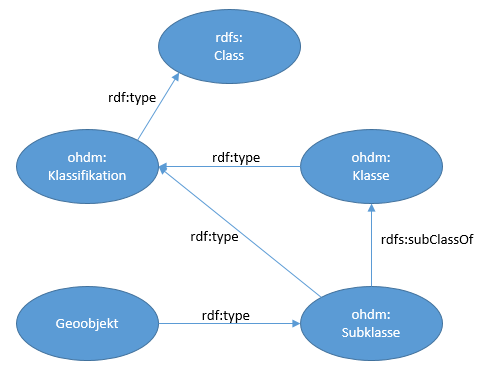
\includegraphics{sparql/ohdm-rdf.PNG}
	\caption{RDF Graph vom OHDM Modell}
	\label{fig:ohdm-rdf}
\end{figure}

\subsection{Schnittstellendefinitionen}

\subsection{genutztes Komponenten}


Den Fuseki Server kann man direkt auf der Homepage jena.apache.org runterladen (aktuelle Version 3.6.0).
Nach dem entpacken muss man den fuseki-server mit chmod die Ausführrechte geben.
Anschließend kann man dann mit ./fuseki-server den Server zum laufen bringen.
Der Server läuft dann standartmäßig auf dem Port 3030 (Portfreigabe erforderlich).
Andere Ports möglich mit ./fuseki-server --port=*number*.

Im Verzeichnis run/ in der Datei shiro.ini kann man die Rechte vergeben.
Standart User, die nicht erstellt werden müssen, sind anon und localhostFilter.
Um die Rechte für jeden Nutzer zu setzen muss man anon bearbeiten.
Um lokal die Rechte zu vergeben bearbeitet man localhostFilter.
Zusätzlich kann man unter [users] eigene Nutzer mit Passwort setzen, den man dann auch Rechte vergeben.

Für die Verbindung zur Datenbank wurde den PostGreSQL Treiber Version 42.1.4 benutz. Die im SQL-Abfrage enthaltene Daten wurden extrahiert und in einem RDF-Modell als Statement hinzugefügt.\newline

Wir haben das Apache Jena Version 3.6.0 benutzt, um RDF-Modelle zu erstellen, zu verwalten und in Dateien zu speichern. Apache Jena ist ein Java-Framework, das umfassende Bibliotheken anbietet mit denen man sehr leicht semantische Anwendungen entwickeln kann.\newline
Mit der SPARQL Bibliothek kann man direkt die RDF Datei abfragen und die Ergebnis anzeigen lassen.

\begin{figure}
	\centering
		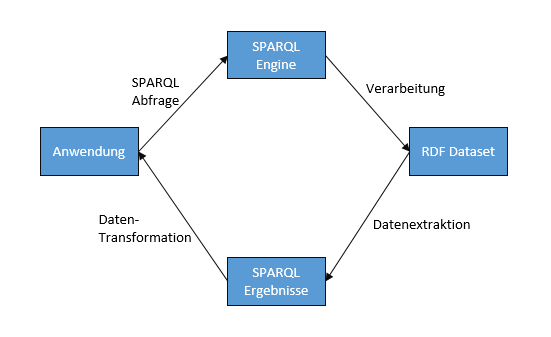
\includegraphics{sparql/sparql-abfrage.PNG}
		\caption{SPARQL Abfrage}
	\label{fig:sparql-abfrage}
\end{figure}

\section{Nutzung}
\subsection{Code}
Der Code befindet sich im SPARQL Repository.

\subsection{Deployment / Runtime}


\section{Qualitätssicherung}


\subsection{Test}


\section{Vorschläge / Ausblick}


